\chapter{Tests and Inference Problems Based on Multinomial Models}

\section{The multinomial model}

Suppose each of $n$ independent units falls into exactly one of $k$ categories, with
probabilities $\theta_1,\dots,\theta_k$ ($\sum\theta_j = 1$). The category counts
$(Y_1,\dots,Y_k)$, $\sum Y_j = n$, have the \emph{multinomial} distribution
\[
\Prob(Y_1=y_1,\dots,Y_k=y_k) = \frac{n!}{y_1!\cdots y_k!}\theta_1^{y_1}\cdots\theta_k^{y_k}.
\]
Each $Y_j\sim\Bin(n,\theta_j)$ marginally.

\begin{theorem}[Multinomial MLE]
The MLEs are $\thetahat_j = y_j/n$.
\end{theorem}
\begin{proof}
Maximize $\ell(\theta) = \sum y_j\log\theta_j$ subject to $\sum\theta_j=1$. With a Lagrange
multiplier, $y_j/\theta_j = \lambda$ for all $j$, so $\theta_j\propto y_j$, and the constraint
gives $\theta_j = y_j/n$.
\end{proof}

\section{Likelihood ratio goodness-of-fit test}

We want to test whether the data are consistent with a hypothesized model
$H_0:\theta_j = \theta_j(\alpha)$ for $j=1,\dots,k$, where $\alpha$ is a vector of $p$
unknown parameters (possibly $p=0$, a completely specified model).

\begin{theorem}[Likelihood ratio GOF statistic]
Let $\hat\alpha$ be the MLE of $\alpha$ under $H_0$ and $e_j = n\,\theta_j(\hat\alpha)$ the
\emph{expected frequencies}. The likelihood ratio statistic is
\[
\Lambda = -2\log\frac{L(\theta(\hat\alpha))}{L(\thetahat)} = 2\sum_{j=1}^k y_j\log\frac{y_j}{e_j}.
\]
Under $H_0$, for large $n$, $\Lambda\approx\chi^2(k-1-p)$.
\end{theorem}
\begin{proof}[Derivation]
$L(\theta)\propto\prod\theta_j^{y_j}$. Unrestricted maximum at $\thetahat_j = y_j/n$; under
$H_0$ at $\theta_j(\hat\alpha) = e_j/n$. So
$\Lambda = 2\sum y_j\big[\log(y_j/n) - \log(e_j/n)\big] = 2\sum y_j\log(y_j/e_j)$. The full
model has $k-1$ free parameters and $H_0$ has $p$, so by the general LRT result the
degrees of freedom are $(k-1)-p$.
\end{proof}

\begin{definition}[Pearson's chi-squared statistic]
\[
D = \sum_{j=1}^k\frac{(y_j-e_j)^2}{e_j},
\]
which is a quadratic approximation to $\Lambda$ (expand $y\log(y/e)$ around $y=e$) and has
the same approximate $\chi^2(k-1-p)$ distribution under $H_0$.
\end{definition}

\textbf{Degrees of freedom:} (number of categories $-1$) $-$ (number of parameters
estimated under $H_0$).
\textbf{Rule of thumb:} the $\chi^2$ approximation is adequate if all $e_j\ge 5$;
otherwise combine adjacent categories. A term $y_j\log(y_j/e_j)$ with $y_j=0$ is
taken as $0$.

\begin{example}[Is the die fair? ($p=0$)]
A die rolled $n=120$ times gives
\begin{center}
\begin{tabular}{lcccccc}
\toprule
face & 1&2&3&4&5&6\\
\midrule
observed $y_j$ & 14 & 23 & 17 & 25 & 16 & 25\\
expected $e_j$ & 20&20&20&20&20&20\\
\bottomrule
\end{tabular}
\end{center}
$H_0:\theta_j = 1/6$ for all $j$, fully specified, so $\text{df} = 6-1-0 = 5$.
\[
D = \frac{36 + 9 + 9 + 25 + 16 + 25}{20} = \frac{120}{20} = 6.00,\qquad
\Lambda = 2\sum y_j\log\frac{y_j}{20} = 6.09.
\]
For $W\sim\chi^2(5)$, $\Prob(W\le 9.236) = 0.90$, so $p>0.10$ (software: $p\approx 0.30$
for both). No evidence that the die is unfair.
\end{example}

\begin{center}
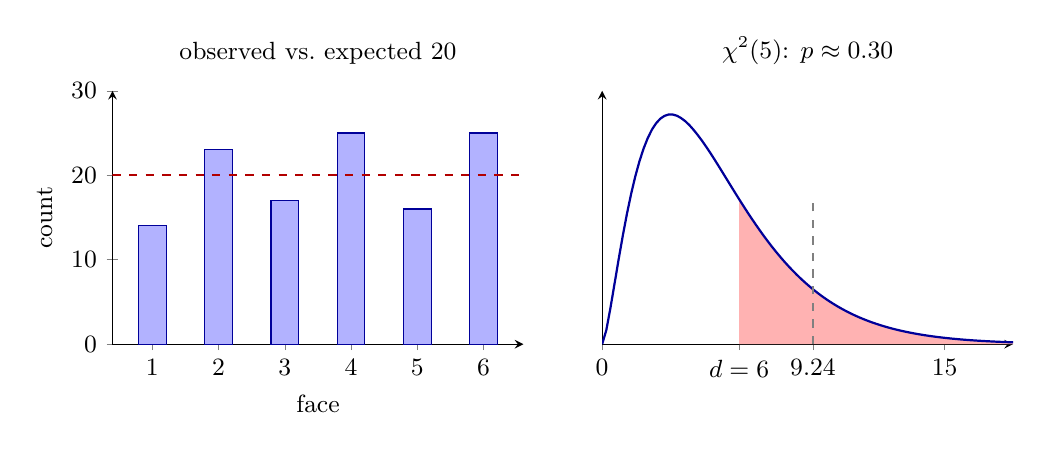
\begin{tikzpicture}
\begin{axis}[name=d1, width=6.8cm, height=4.8cm, ybar, bar width=10pt, ymin=0, ymax=30, xtick={1,...,6},
    xlabel={face}, ylabel={count}, tick label style={font=\small}, label style={font=\small}, axis lines=left, scaled y ticks=false, yticklabel style={/pgf/number format/fixed}, enlarge x limits=0.12, title={observed vs.\ expected $20$},
    title style={font=\small}]
  \addplot[fill=blue!30, draw=blue!60!black] coordinates {(1,14) (2,23) (3,17) (4,25) (5,16) (6,25)};
  \draw[thick, dashed, red!70!black] (axis cs:0.4,20) -- (axis cs:6.6,20);
\end{axis}
\begin{axis}[at={(d1.east)}, anchor=west, xshift=1cm, width=6.8cm, height=4.8cm, xmin=0, xmax=18,
    ymin=0, ymax=0.17, ytick=\empty, xtick={0,6,9.236,15}, xticklabels={0,$d=6$,$9.24$,15}, tick label style={font=\small}, label style={font=\small}, axis lines=left, scaled y ticks=false, yticklabel style={/pgf/number format/fixed},
    samples=100, title={$\chi^2(5)$: $p\approx0.30$}, title style={font=\small}]
  \addplot[draw=none, fill=red!30, domain=6:18] {x^1.5*exp(-x/2)/7.5199} \closedcycle;
  \addplot[thick, blue!60!black, domain=0:18] {x^1.5*exp(-x/2)/7.5199};
  \draw[dashed, gray] (axis cs:9.236,0) -- (axis cs:9.236,0.1);
\end{axis}
\end{tikzpicture}
\end{center}
The deviations from $20$ (left) are of the size chance produces: the observed $d = 6$ sits
in the bulk of the $\chi^2(5)$ distribution (right), well below the $10\%$ point $9.236$.

\begin{example}[Poisson goodness of fit ($p=1$)]
The car counts of Chapter 2 in $n=200$ intervals had observed frequencies
$38,80,50,20,12$ for $0,1,2,3,\ge4$ cars, $\thetahat = 1.455$ and expected frequencies
$46.68, 67.92, 49.41, 23.96, 12.02$ (all $\ge 5$). The contributions to $D$ are
\[
\frac{(38-46.68)^2}{46.68} = 1.614,\ \ 2.149,\ \ 0.007,\ \ 0.656,\ \ 0.000,
\]
so $D = 4.43$; similarly $\Lambda = 2\sum y_j\log(y_j/e_j) = 4.46$. Degrees of freedom:
$5 - 1 - 1 = 3$ (one parameter $\theta$ was estimated). For $W\sim\chi^2(3)$,
$\Prob(W\le 6.251) = 0.90$, so $p>0.10$ (software $p\approx0.22$). No evidence against the
Poisson model.
\end{example}

\section{Two-way tables and tests of independence}

Each of $n$ units is classified by two categorical variates $A$ (with $a$ levels) and $B$
(with $b$ levels), giving counts $y_{ij}$ in an $a\times b$ \emph{contingency table}, with
row totals $r_i = \sum_j y_{ij}$ and column totals $c_j = \sum_i y_{ij}$.

Model: multinomial with cell probabilities $\theta_{ij}$, $ab-1$ free parameters.
The hypothesis of \emph{independence} of $A$ and $B$ is
\[
H_0:\theta_{ij} = \alpha_i\beta_j\quad\text{for all } i,j,
\]
with $\sum\alpha_i = \sum\beta_j = 1$, i.e.\ $(a-1)+(b-1)$ free parameters.

\begin{theorem}[Test of independence]
Under $H_0$ the MLEs are $\hat\alpha_i = r_i/n$, $\hat\beta_j = c_j/n$, so the expected
frequencies are
\[
e_{ij} = n\hat\alpha_i\hat\beta_j = \frac{r_i c_j}{n}.
\]
The statistics $\Lambda = 2\sum_{i,j}y_{ij}\log(y_{ij}/e_{ij})$ and
$D = \sum_{i,j}(y_{ij}-e_{ij})^2/e_{ij}$ are approximately $\chi^2\big((a-1)(b-1)\big)$ under
$H_0$, since $(ab-1) - (a-1) - (b-1) = (a-1)(b-1)$.
\end{theorem}

\begin{remark}
The same computation tests \emph{homogeneity}: if $a$ separate random samples are taken
(e.g.\ fixed numbers of men and women) and each classified by $B$, the hypothesis that the
$B$-distribution is the same in all $a$ populations leads to identical $e_{ij}$, statistic
and degrees of freedom.
\end{remark}

\begin{example}[$2\times3$ table]
A random sample of $250$ students classified by faculty and preferred course format:
\begin{center}
\begin{tabular}{lcccc}
\toprule
 & online & hybrid & in person & total\\
\midrule
Math & 60 \ (48) & 45 \ (48) & 15 \ (24) & 120\\
Arts & 40 \ (52) & 55 \ (52) & 35 \ (26) & 130\\
\midrule
total & 100 & 100 & 50 & 250\\
\bottomrule
\end{tabular}
\end{center}
Expected frequencies in parentheses, e.g.\ $e_{11} = 120(100)/250 = 48$,
$e_{13} = 120(50)/250 = 24$. The contributions to $D$ are
\[
\begin{array}{ccc}
3.000 & 0.188 & 3.375\\
2.769 & 0.173 & 3.115
\end{array}
\]
so $D = 12.62$ (and $\Lambda = 12.86$), with $(2-1)(3-1) = 2$ degrees of freedom. For
$W\sim\chi^2(2)$, $\Prob(W\le 9.210) = 0.99$, so $p<0.01$ (software: $p\approx0.002$). Strong
evidence that format preference is associated with faculty: Math students prefer online
more, Arts students prefer in-person more than independence predicts.
\end{example}

\begin{center}
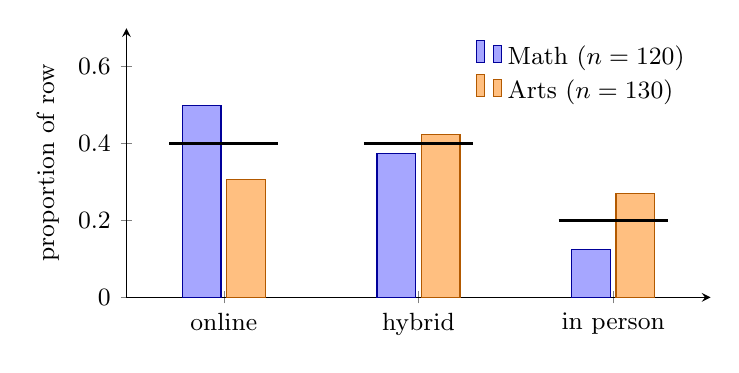
\begin{tikzpicture}
\begin{axis}[width=9cm, height=5cm, ybar, bar width=14pt, ymin=0, ymax=0.7, xtick={1,2,3},
    xticklabels={online, hybrid, in person}, ylabel={proportion of row}, tick label style={font=\small}, label style={font=\small}, axis lines=left, scaled y ticks=false, yticklabel style={/pgf/number format/fixed}, enlarge x limits=0.25,
    legend style={font=\small, draw=none}, legend cell align=left]
  \addplot[fill=blue!35, draw=blue!60!black] coordinates {(1,0.5) (2,0.375) (3,0.125)};
  \addplot[fill=orange!50, draw=orange!70!black] coordinates {(1,0.3077) (2,0.4231) (3,0.2692)};
  \draw[very thick] (axis cs:0.72,0.4) -- (axis cs:1.28,0.4);
  \draw[very thick] (axis cs:1.72,0.4) -- (axis cs:2.28,0.4);
  \draw[very thick] (axis cs:2.72,0.2) -- (axis cs:3.28,0.2);
  \legend{Math ($n=120$), Arts ($n=130$)}
\end{axis}
\end{tikzpicture}
\end{center}
Under independence both faculties would match the overall column proportions (black lines:
$0.4$, $0.4$, $0.2$). Math leans online and Arts leans in-person, which is the pattern
the test detects.

\begin{example}[$2\times2$ table]
Of $50$ patients on treatment A, $30$ improved; of $50$ on treatment B, $18$ improved.
Totals: $48$ improved, $52$ did not. Expected: $e = 50(48)/100 = 24$ improved and $26$ not,
in each group. Then
\[
D = \frac{6^2}{24}+\frac{6^2}{26}+\frac{6^2}{24}+\frac{6^2}{26} = 1.5 + 1.385 + 1.5 + 1.385 = 5.77,
\]
on $1$ degree of freedom; $p = \Prob(W\ge 5.77) = \Prob(|Z|\ge 2.40) \approx 0.016$
($\Lambda = 5.83$ gives $p\approx 0.016$ too). Evidence that improvement rates differ.
(For a $2\times2$ table this is equivalent to the two-sided test comparing two binomial
proportions.)
\end{example}

\begin{important}[Common pitfalls]
\begin{itemize}
  \item Use \emph{counts}, never percentages, in $D$ and $\Lambda$.
  \item Subtract one degree of freedom for each parameter estimated from the data under
        $H_0$.
  \item Check $e_j\ge5$; merge sparse categories before testing.
  \item A significant test of independence shows association, not causation.
  \item These tests are always ``one-tailed'' in the sense that only large $D$ counts as
        evidence against $H_0$.
\end{itemize}
\end{important}

\section*{Summary}
\begin{itemize}
  \item Multinomial MLE: $\thetahat_j = y_j/n$.
  \item Goodness of fit: $\Lambda = 2\sum y_j\log(y_j/e_j)$ or $D = \sum(y_j-e_j)^2/e_j$,
        approximately $\chi^2(k-1-p)$.
  \item Independence in an $a\times b$ table: $e_{ij} = r_ic_j/n$, $\chi^2((a-1)(b-1))$.
\end{itemize}
